%%% License: Creative Commons Attribution Share Alike 4.0 (see https://creativecommons.org/licenses/by-sa/4.0/)

\documentclass[english,10pt
,aspectratio=169
%,handout
%%%%%,notes
]{beamer}
%%% License: Creative Commons Attribution Share Alike 4.0 (see https://creativecommons.org/licenses/by-sa/4.0/)

\DeclareGraphicsExtensions{.eps, .pdf,.png,.jpg,.mps,}
\usetheme{reMedian}
\usepackage{parskip}
\makeatother

\renewcommand{\baselinestretch}{1.1} 

\usepackage{amsmath, amssymb, amsfonts, amsthm}
\usepackage{enumerate}
%\usepackage{enumitem}
\usepackage{hyperref}
\usepackage{url}
\usepackage{bbm}
\usepackage{color}

\usepackage{tikz}
\usepackage{tikzscale}
\newcommand*\circled[1]{\tikz[baseline=(char.base)]{
		\node[shape=circle,draw, inner sep=-20pt] (char) {#1};}}
\usetikzlibrary{automata,positioning}
\usetikzlibrary{decorations.pathreplacing}
\usepackage{pgfplots}
\usepgfplotslibrary{fillbetween}
\usepackage{graphicx}

\usepackage{setspace}
\thinmuskip=1mu
\medmuskip=1mu 
\thickmuskip=1mu 


\usecolortheme{default}
\usepackage{verbatim}
\usepackage[normalem]{ulem}

\usepackage{apptools}
\AtAppendix{
	\setbeamertemplate{frame numbering}[none]
}
\usepackage{natbib}


% red strikeout
\newcommand\soutred{\bgroup\markoverwith
	{\textcolor{red}{\rule[0.55ex]{2pt}{0.8pt}}}\ULon}



% To use LyX frames from old version:
\def\lyxframeend{} % In case there is a superfluous frame end
\long\def\lyxframe#1{\@lyxframe#1\@lyxframestop}%
\def\@lyxframe{\@ifnextchar<{\@@lyxframe}{\@@lyxframe<*>}}%
\def\@@lyxframe<#1>{\@ifnextchar[{\@@@lyxframe<#1>}{\@@@lyxframe<#1>[]}}
\def\@@@lyxframe<#1>[{\@ifnextchar<{\@@@@@lyxframe<#1>[}{\@@@@lyxframe<#1>[<*>][}}
\def\@@@@@lyxframe<#1>[#2]{\@ifnextchar[{\@@@@lyxframe<#1>[#2]}{\@@@@lyxframe<#1>[#2][]}}
\long\def\@@@@lyxframe<#1>[#2][#3]#4\@lyxframestop#5\lyxframeend{%
	\frame<#1>[#2][#3]{\frametitle{#4}#5}}


\title{Mechanism Design}

\subtitle{1: Definitions, Implementation}

\author{Egor Starkov}

\date{K{\o}benhavns Unversitet \\
	Fall 2022}


\begin{document}
	\AtBeginSection[]{
		\frame{
			\frametitle{This slide deck:}
			\tableofcontents[currentsection,currentsubsection]
	}}
	\frame[plain]{\titlepage}

\note{
	\begin{itemize}
		\item Last time we talked about seemingly nothing at all. Some concepts, some logistics, some introductions and technical difficulties -- and we finished early.
		\item We actually covered some core ideas and concepts. Today we will define those concepts formally.
		\item It will seem like repetition. But it's not.
		When you want to draw a plot in mathematica -- you know that `x' is a variable that should be on horizontal axis. But the computer does not. You need to put a line of code saying ``x is a variable''. Math is like computer. To use all the cool stuff from future lectures we need to introduce all the formal mathematical objects that it can work with. Today we'll do that.
		\item %2020 only
		Question last time: what's the line between CT and MD? MD is focused on shaping \emph{interactions} between many agents.
	\end{itemize}
}



%\begin{frame}
%	(math exercise from notes)
%\end{frame}
%\note{
%	\begin{itemize}
%		\item asked to read mathreview -- how many did that?
%		\begin{itemize}
%			\item introduce quick survey protocol (1s in chat)
%		\end{itemize}
%		\item $\int_a^b x^2 \log (x) dx$: $u=\log(x)$, $dv = x^2 dx$, so $du = 1/x dx$, $v = \frac{x^3}{3}$ and
%		\begin{align*}
%			\int_a^b x^2 \log (x) dx 
%			&= \left(\frac{x^3}{3}\log(x) \right)|_a^b - \int_a^b \frac{x^2}{3} dx
%			\\
%			&= \left(\frac{x^3}{3}\log(x) - \frac{x^3}{9} \right)|_a^b
%		\end{align*}
%	\end{itemize}
%}


\section{Defining a Mechanism}

\begin{frame}{What is a mechanism?}
	Let's reverse engineer from a simpler question:
	\textbf{What is a game?}
	\begin{enumerate}
		\item Set of players $i \in\{ 1,...,N\}$
		\item Set of actions $A_i$ for every $i$; set of action profiles $A \equiv \times_{i \in N} A_i$
		\item Collection of utility functions $u_i: A \to \mathbb{R}$
	\end{enumerate}
	(This is a \emph{normal-form game}. All extensive-form games (``trees'') and incomplete-information games can be represented as normal-form games.)
	
	Which parts of this definition are fixed at a higher level, and which can we \emph{design} as a part of a \emph{mechanism}?
\end{frame}


\begin{frame}{Problem environment}
	\centering
	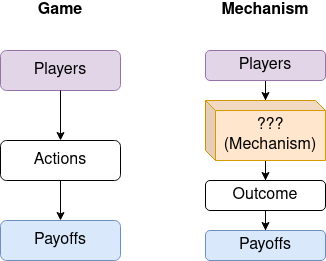
\includegraphics[scale=0.7]{pics/M1/game_vs_mech}
\end{frame}


\begin{frame}{General Problem Set-up}
	In our MD problem, the following environment will be \textbf{fixed}:
	\begin{itemize}
		\item $N$ agents,
		\item set $X$ of \alert{outcomes},
		\item each agent $i$ has \alert{type} $\theta_i\in\Theta_{i}$:
		\begin{itemize}
			\item describes agent's \structure{information},
			\item describes agent's \structure{preferences};
		\end{itemize}
		\item the type profile $\theta=(\theta_1,\dots,\theta_{N})$ is distributed according to a distribution $F$ with p.d.f. $\phi$,
		\begin{itemize}
			\item (often a missing subscript denotes a vector of respective objects)
			\item distribution $F$ is commonly known and agreed upon
		\end{itemize}
		\item each agent has a \alert{utility} function $u_{i}(x,\theta_{i})$ that depends on the collective choice $x \in X$ and his type $\theta_i$,
	\end{itemize}
\end{frame}


\begin{frame}{Social Choice Function}
	\begin{definition}[Social choice function]
		A \alert{social choice function} is a function \alert{$f:\Theta_{1}\times \dots\times\Theta_{N}\rightarrow X$} that assigns to each profile of types $(\theta_{1},\dots,\theta_{N})$ a collective choice $f(\theta_{1},\dots,\theta_{N})\in X$.
	\end{definition}
	\begin{itemize}
		\item gives a desired outcome as a function of the agents' types
	\end{itemize}
\end{frame}


\begin{frame}{Mechanism}
	\begin{itemize}
		\item a mechanism is a game played by the agents
		\item each agent has an action set $A_{i}$ in this game
	\end{itemize}
	\begin{definition}[mechanism]
		A \alert{mechanism} $\Gamma=(A_{1},\dots,A_{N},g(\cdot))$ is a collection of: 
		\begin{itemize}
			\item N \structure{strategy sets} $(A_{1},\dots,A_{N})$ and 
			\item an \structure{outcome function} $g:A_{1}\times\dots\times A_{N}\rightarrow X$.
		\end{itemize}
	\end{definition}
\end{frame}


\begin{frame}{Implementation}
	\begin{definition}[implementation]
		Mechanism $\alert{\Gamma}=(A_{1},\dots,A_{N},g(\cdot))$ \alert{implements} the s.c.f. $\alert{f}$ if there is \structure{an equilibrium} strategy profile $(a_{1}^{*},\dots,a_{N}^{*})$ of the Bayesian game induced by $\Gamma$ \structure{such that} 
		$$\structure{g}(a_{1}^{*}(\theta_{1}),\dots,a_{N}^{*}(\theta_{N})) = \structure{f} (\theta_{1},\dots,\theta_{N})$$ 
		for all $(\theta_{1},\dots,\theta_{N})\in\Theta_{1}\times\dots \times\Theta_{N}$.
	\end{definition}
\end{frame}


\begin{frame}{Summary of definitions}
	\begin{itemize}
		\item S.c.f. $f$ describes what we want to achieve;
		\item Mechanism $\Gamma = (S,g)$ describes what we do and how;
		\item Implementability says whether we have achieved our goal.
	\end{itemize}
\end{frame}


\begin{frame}{Full problem setup}
	\centering
	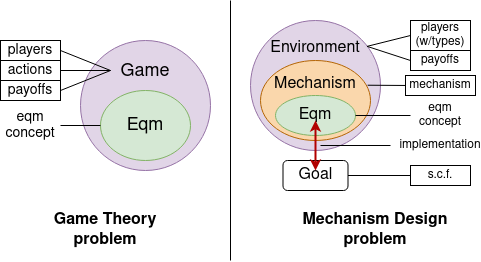
\includegraphics[scale=0.7]{pics/M1/game_vs_mech2}
\end{frame}


%\begin{frame}
%	(mechanism proposals)
%\end{frame}



\section{Revelation Principle}

\begin{frame}{Revelation Principle}
	\begin{itemize}
		\item Main cheat in Mechanism Design! No need to bruteforce through uncountable numbers of different games! It is enough to just... \only<1>{(\href{https://www.youtube.com/watch?v=dQw4w9WgXcQ}{{click to see more}})}
		\pause
		\item Instead of making players play the game, ask them for their $\theta_i$ and promise to play on their behalf!
		\item Requires that the designer has commitment power.
		\begin{itemize}
			\item Strong assumption, sometimes reasonable(?)
			\item The necessary evil for our purposes.
		\end{itemize}
	\end{itemize}
\end{frame}


\begin{frame}{Revelation Principle: Definitions}
	Fix some s.c.f. $f:\Theta \to X$.
	\begin{definition}[Direct revelation mechanism]
		A \structure{direct revelation mechanism} for $f$ is a mechanism in which $A_i = \Theta_i$ for all $i$ and $g(\theta) = f(\theta)$
	\end{definition}
	
	\begin{definition}[Truthuful implementation]
		S.c.f. $f$ is \structure{truthfully implementable} if it can be implemented by a direct revelation mechanism.
	\end{definition}
\end{frame}


\begin{frame}{Revelation Principle: Statement}
	\begin{block}{Revelation principle (blanket statement)}
		Suppose there exists a mechanism $\Gamma=(A_{1},\dots,A_{N},g)$ that implements the social choice function $f$.\\ Then $f$ is \structure{truthfully implementable}.
	\end{block}
	\medskip
	\begin{itemize}
		\item The ``theorem'' above is informal.
		\begin{itemize}
			\item ``Implementation'' requires ``an equilibrium'', which can mean a million different things.
			\item We will now plug in some specific equilibrium concepts.
		\end{itemize}
	\end{itemize}
\end{frame}
\note{
	\begin{itemize}
		\item We cannot fool agents by designing a very complicated game -- because they are rational and will compute the optimal strategy regardless
		\begin{itemize}
			\item This is, in part, to impose discipline our models -- if can deceive or confuse players then why not just do that.
			\item Economics is the science about being ``technically truthfull'' -- can never lie in equilibrium.
		\end{itemize}
		\item We need a formal equilibrium concept, so let's introduce one...
		\begin{itemize}
			\item Who knows which eqm concepts?
		\end{itemize}
	\end{itemize}
}




\section{Dominant Strategy Implementation}

%TODO 2020: switch from s and S to a and A since there are all actions, not strategies.
%TODO2021: was that the right call?
\begin{frame}{Recap: Dominant Strategy}
	\begin{itemize}
		\item strategy $a_i$ is a full contingent plan of play
		\item strategy $a_i$ is \alert{dominant} for agent $i$ if it is best \emph{no matter what the other players do}
	\end{itemize}
	\begin{definition}[dominant strategy]
		Given mechanism $\Gamma=(A,g)$,
		$a_{i}: \Theta_{i}\rightarrow A_{i}$ is a \structure{dominant strategy} if for all $\theta_{i}\in \Theta_{i}$
		$$ u_{i}(g(a_{i}(\theta_{i}),a_{-i}),\theta_{i})\geq u_{i}(g(\hat a_{i},a_{-i}),\theta_{i})$$
		for all $\hat a_{i}\in A_{i}$  and all $a_{-i}\in A_{-i}$.
	\end{definition}
	\begin{itemize}
		\item our definition slightly different from the standard -- does not require strict inequality
	\end{itemize}
\end{frame}


\begin{frame}{Dominant Strategy Equilibrium}
	\begin{itemize}
		\item in a \alert{dominant strategy equilibrium} every player plays a dominant strategy
	\end{itemize}
	\begin{definition}[dominant strategy equilibrium]
		A strategy profile $(a_1^*,\dots,a_N^*)$ is a \structure{dominant strategy equilibrium} of mechanism  $\Gamma=(A_{1},\dots,A_{N},g)$ if for all $i$ and all $\theta_{i}\in \Theta_{i}$
		$$ u_{i}(g(a_{i}^{*}(\theta_{i}),a_{-i}),\theta_{i}) \geq u_{i}(g(\hat a_{i},a_{-i}), \theta_{i})$$
		for all $\hat a_{i}\in A_{i}$ and all $a_{-i}\in A_{-i}$.
	\end{definition}

	Now let's finally be formal about all our definitions.
\end{frame}


\begin{frame}{Dominant Strategy Implementation}
	\begin{itemize}
		\item A mechanism \alert{implements $f$ in dominant strategies} if
		\begin{itemize}
			\item the game induced by the mechanism has a dominant strategy equilibrium
			\item the outcome in this equilibrium coincides with $f$
		\end{itemize}
	\end{itemize}
	\begin{definition}[implementation in dominant strategies]
		A mechanism $\Gamma=(A_{1},\dots,A_{N},g)$ \structure{implements} the social choice function $f$ \structure{in dominant strategies} if there exists a dominant strategy equilibrium $(a_1^*,\dots,a_N^*)$ of $\Gamma$ such that $g(a_1^*(\theta_{1}),\dots,a_N^*(\theta_{N}))=f(\theta)$ for all $\theta\in\Theta$.
	\end{definition}
\end{frame}


\begin{frame}{Good Implementation Concept?}
	\begin{itemize}
		\item very robust equilibrium concept
		\begin{itemize}
			\item no need to predict what the other players will play
			\item no need to know the type distribution $\phi$
			\item works even if
			\begin{itemize}
				\item players don't know $\phi$ or even if players believe in different $\phi_{i}$ (protects from players' model misspecification)
				\item players think that other players are not rational
			\end{itemize}
		\end{itemize}
		\item not a panacea
		\begin{itemize}
			\item does not rule out other weird Nash Equilibria (remember SPA)
			\item is not necessarily collusion-proof
			\item does not protect from designer's model misspecification
		\end{itemize}
	\end{itemize}
	Bottom line: it's as good as they get, but far from perfect.
\end{frame}


\begin{frame}{Dominant Strategy Incentive Compatibility}
	\begin{theorem}[Revelation Principle for Dominant Strategies]
		Suppose there exists a mechanism $\Gamma=(A_{1},\dots,A_{N},g)$ that implements the social choice function $f$ in dominant strategies.\\ Then $f$ is \structure{truthfully implementable} in dominant strategies.
	\end{theorem}
	\medskip
	\begin{definition}[Dominant Strategy Incentive Compatibility]
		``$f$ is \alert{dominant strategy incentive compatible} (DSIC)''\\ 
		means the exact same thing as \\
		``$f$ is \structure{truthfully implementable in dominant strategies}''.
	\end{definition}
\end{frame}


\begin{frame}{DS Revelation Principle: Proof}
	Let $\Gamma$ implement $f$ in dominant strategies, i.e. there is a strategy profile  $(a_1^*,\dots,a_N^*)$ such that $g(a_1^*(\theta_{1}),\dots,a_N^*(\theta_{N}))=f(\theta)$ for all $\theta$, and for all $i$ and  $\theta_{i}\in\Theta_{i}$,
	$$ u_{i}(g(a_{i}^{*}(\theta_{i}),a_{-i}),\theta_{i})\geq u_{i}(g(\hat a_{i},a_{-i}),\theta_{i})$$
	for all $\hat a_{i}\in A_{i}$ and all $a_{-i}\in A_{-i}$. 
	
	Then
	$$ u_{i}(g(a_{i}^{*}(\theta_{i}), a_{-i}^{*}(\theta_{-i})),\theta_{i})\geq u_i (g(a^*_i(\hat{\theta}_i), a_{-i}^{*}(\theta_{-i})), \theta_i)$$
	for all $\hat{\theta}_i \in \Theta_i$, $\theta_{-i} \in \Theta_{-i}$. 
	
	Since $g(a^*(\theta)) = f(\theta)$,
	$$ u_i (f(\theta_i,\hat{\theta}_{-i}),\theta_i) \geq u_i (f(\hat{\theta}_i,\hat{\theta}_{-i}), \theta_i)$$
	for all $\hat{\theta}_{-i} \in \Theta_{-i}$.
\end{frame}
\note{
	Main idea: we have IC constraints for the original mechanism. Want to show that IC constraints for a DRM will also hold.
}


\begin{frame}{Revelation Principle: Is it cool or is it cool?}
	\begin{itemize}
		\item Idea: to solve the problem \structure{mathematically}, it is enough to only look at \structure{direct mechanisms}!
		\begin{itemize}
			\item This result allows to quickly check whether a given $f$ is [DS] implementable.
			\item If yes, gives you a mechanism to implement it.
			\item If not, helps you describe a set of implementable s.c.f. and pick second best.
			\item \emph{Yours today for \soutred{only \$49.99+shipping} FREE with a qualifying Mechanism Design course!}
		\end{itemize}
		\item Translating that solution to \alert{the real world} may (and often does) result in an \alert{indirect mechanism}! We'll see some examples.
	\end{itemize}
\end{frame}


\section{Bayesian Implementation}

\begin{frame}{DSIC vs BIC}
\begin{itemize}
	\item We've looked at DS implementation so far. Robust but demanding. Can we get more mileage by relaxing the equilibrium notion?
	\item Now: use standard \structure{Bayes-Nash Equilibrium} as solution concept. Weaker equilibrium concept, so:
	\begin{itemize}
		\item we are less confident it will produce the intended outcome, but
		\item it can implement more(?) s.c.f-ns. 
		\item (there's a literature studying whether sets of DSIC and BIC s.c.f-ns are equal in special settings)
	\end{itemize}
	%\item Now prior $\phi$ about the distribution of types becomes more relevant (though we already used it when talking about revenue)
\end{itemize}
\end{frame}
\note{(video script):
So far we have talked about dominant strategy implementation. This is a strong implementation concept, but not the only one. Today we will introduce another one of those, called Bayesian implementation.
}


\begin{frame}{Bayesian Implementation}
Start with the \alert{general model} as before:
\begin{itemize}
	\item $N$ agents;
	\item set of alternatives $X$;
	\item type $\theta_{i}\in\Theta_{i}$ is private information of $i$;
	\item common prior belief $\phi \in \varDelta(\Theta)$ about distribution of types;
	\item utility functions $u_i(x,\theta_i)$;
	\item each agent uses Bayes' rule to form a belief over other agents' types\\
	$$\phi(\theta_{-i}|\theta_{i}) = \phi(\theta_{i},\theta_{-i}|\theta_{i}) = \frac{\phi(\theta_{i}, \theta_{-i}) }{\int_{\tilde\theta_{-i}\in\Theta_{-i}} \phi(\theta_{i},\tilde\theta_{-i}) d\tilde{\theta}_{-i}}.$$
\end{itemize}
\end{frame}
\note{(video script):
In particular, this framework is defined in terms of a set of agents, a set of types for every agent, an arbitrary set of outcomes that we are choosing among (coupled with a s.c.f., which I did not write down), and a common prior belief over type profiles, shared by all agents.
We also have agents' utility functions that map outcomes and type profiles into utility values.

With Bayesian Implementation, we take an interim perspective, rather than ex post perspective in case of DS implementation, meaning that we now have to keep track of the beliefs that every type of every player has about other players' types. To that end, we assume that all players start with a common prior belief over type profiles and then employ Bayes' rule to update this belief once they observe their own type.

In particular, Bayes' rule says that the probability $\phi$ that
player $i$ assigns to profile of other players' types $\theta_{-i}$
given their own type $\theta_{i}$ is given by the ratio of: the joint
probability of types $\theta_{i}$ and $\theta_{-i}$ occuring simultaneously
and the total probability of type $\theta_{i}$ occurring, which is
given by the integral of the p.d.f. $\phi(\theta)$ over all possible
profiles of other players' types, $\tilde{\theta}_{-i}$.

Now that we have defined the setting we work in, the next step towards
introducing an implementation concept, is introducing the equilibrium
concept that will be used in this implementation concept.
}


\begin{frame}{Bayes-Nash Equilibrium}
\begin{definition}[Bayes-Nash equilibrium]
	The \structure{strategy profile} $a^* =(a_{1}^*,\dots,a_{N}^*)$ with $a_i^*: \Theta_i \to A_i$ is a \alert{Bayes-Nash equilibrium} of the mechanism $\Gamma=(A_{1},\dots,A_{N},g)$ if, for all $i$ and all $\theta_{i}\in\Theta_{i}$,
	$$E_{\theta_{-i}}\left[u_{i}(g(a_i^*(\theta_i),a_{-i}^*(\theta_{-i})),\theta_{i})|\theta_{i}\right]\geq E_{\theta_{-i}}\left[u_{i}(g(\hat a_i,a_{-i}^*(\theta_{-i})),\theta_{i})|\theta_{i}\right]$$
	for all $\hat a_{i}\in A_{i}$.
\end{definition}
\pause
\begin{itemize}
	\item Standard NE reasoning: if everyone else plays eqm strats, $i$ has no incentive to deviate.
	\item (This definition is for pure strategies, but there is no problem in allowing mixed strategies.)
	\item Expectations are taken w.r.t. distribution $F(\theta)$
	\item BTW: we assumed that allocation and transfers are \emph{deterministic} given reports. \href{https://doi.org/10.3982/ECTA14698}{\uline{Chen, He, Li, and Sun (2019)}} show that this is often without loss of generality.
\end{itemize}
\end{frame}
\note{(video script):
The equilibrium concept we will be using here is Bayes-Nash Equilibrium.
This equilibrium is composed by a strategy profile $a^{*}$, -- where
each player's strategy maps their types into their action set, which
is prescribed by the mechanism, -- and this strategy profile is such
that every type of every player must find it optimal to play the equilibrium
action rather than any other action.

The utility here comes from the outcome implemented following a given
action profile, according to the outcome function $g$, which is specified
as a part of the mechanism. The agents' decision criterion that we
employ here is expected utility, where the expectation is taken over
other players' types $\theta_{-i}$, which are not known to agent
$i$ when he selects an action, and the expectation is taken w.r.t.
agent $i$'s belief that we have just seen.
}



\begin{frame}{Bayesian Implementation}
\begin{definition}[Bayesian implementation]
	\structure{Mechanism} $\Gamma=(A_{1},\dots,A_{N},g)$ \alert{implements \structure{s.c.f. $f$} in Bayes-Nash equilibrium} if there is a BNE $a^*=(a_{1}^*,\dots,a_{N}^*)$ of $\Gamma$ such that $f(\theta)=g(a^{*}(\theta))$ for all $\theta\in \Theta$.
\end{definition}
\pause
\begin{definition}[Bayesian implementability]
	\structure{S.c.f. $f$} is \alert{implementable in BNE} if there exists $\Gamma$ which implements it in BNE.
\end{definition}
\end{frame}
\note{(video script):
Now that we have our equilibrium concept, we can introduce the implementation
concept.

We will say that mechanism $\Gamma$ implements s.c.f. $f$ in Bayes-Nash
equilibrium if the game induced by mechanism $\Gamma$ has a BNE that
leads to the same outcome as the one prescribed by $f$, for any type
profile $\theta$.

We will then say that a social choice function $f$ is implementable
in BNE if there exists some mechanism $\Gamma$ that implements it
in BNE. To clarify, the first definition has to do with whether a
given mechanism $\Gamma$ implements a given s.c.f., while the second
definition asks whether there is any mechanism $\Gamma$ that implements
a given s.c.f..
}


\begin{frame}{Truthful Bayesian Implementation}
\begin{definition}[Truthful Bayesian implementation]
	\structure{S.c.f. $f$} is \alert{truthfully implementable in BNE} (=Bayesian Incentive Compatible, \alert{BIC}) if $a_{i}^*(\theta_{i})=\theta_{i}$ is a BNE of the direct revelation mechanism $\Gamma=(\Theta_{1},\dots,\Theta_{N},f)$. 
	\bigskip
	
	That is, for all $i,\theta_{i}$, and $\hat{\theta}_{i}\in\Theta_{i}$,
	\vspace{-0.5em}\begin{align*}
		E_{\theta_{-i}}\left[u_{i}(f(\theta_i,\theta_{-i}),\theta_{i})|\theta_{i}\right]\geq E_{\theta_{-i}}\left[u_{i}(f(\hat \theta_{i},\theta_{-i}),\theta_{i})|\theta_{i}\right].
	\end{align*}\vspace{-1em}
\end{definition}
Every player is asked for their type; reporting truthfully is a BNE.
\end{frame}
\note{(video script):
Now that we have introduced our new implementation concept, we can
also restate the revelation principle for Bayesian mechanisms. The
first definition on this path is that of truthful implementation.

In particular, we will call a given s.c.f. truthfully implementable
in BNE or, as we will call it more often, Bayesian Incentive Compatible,
if it is implemented in BNE by a DRM -- meaning that truthful reporting
is a BNE of the direct revelation mechanism for this s.c.f..

In other words, scf $f$ is BIC if the following condition holds: ...

for all players and their types, the
expected utility from reporting own type truthfully to the mechanism
is at least as large as from any possible misreport.
}


\begin{frame}{Revelation principle}
\begin{theorem}[Revelation principle for Bayes-Nash equilibrium]
	\structure{If} there exists a mechanism $\Gamma=(A_{1},\dots,A_{N},g)$ that \structure{implements} $f$ in BNE, 
	\alert{then} $f$ is \alert{truthfully implementable} in BNE.
\end{theorem}

The proof is pretty much the same as for DSIC.
\end{frame}
\note{(video script):
Now we state the revelation principle.

Its statement is analogous to the revelation principle for DSIC mechanisms. It says that if some scf f is implemented by some mechanism $\Gamma$ in BNE then it can also be implemented in BNE by a direct mechanism.

The proof of the statement is completely analogous to the proof for dominant strategies and consists of showing that if Bayesian IC constraints are satisfied for some mechanism then they would also be satisfied for a direct mechanism. We will therefore not go through this proof in detail.
}



\end{document}